
\begin{figure}[hp]

\hfil
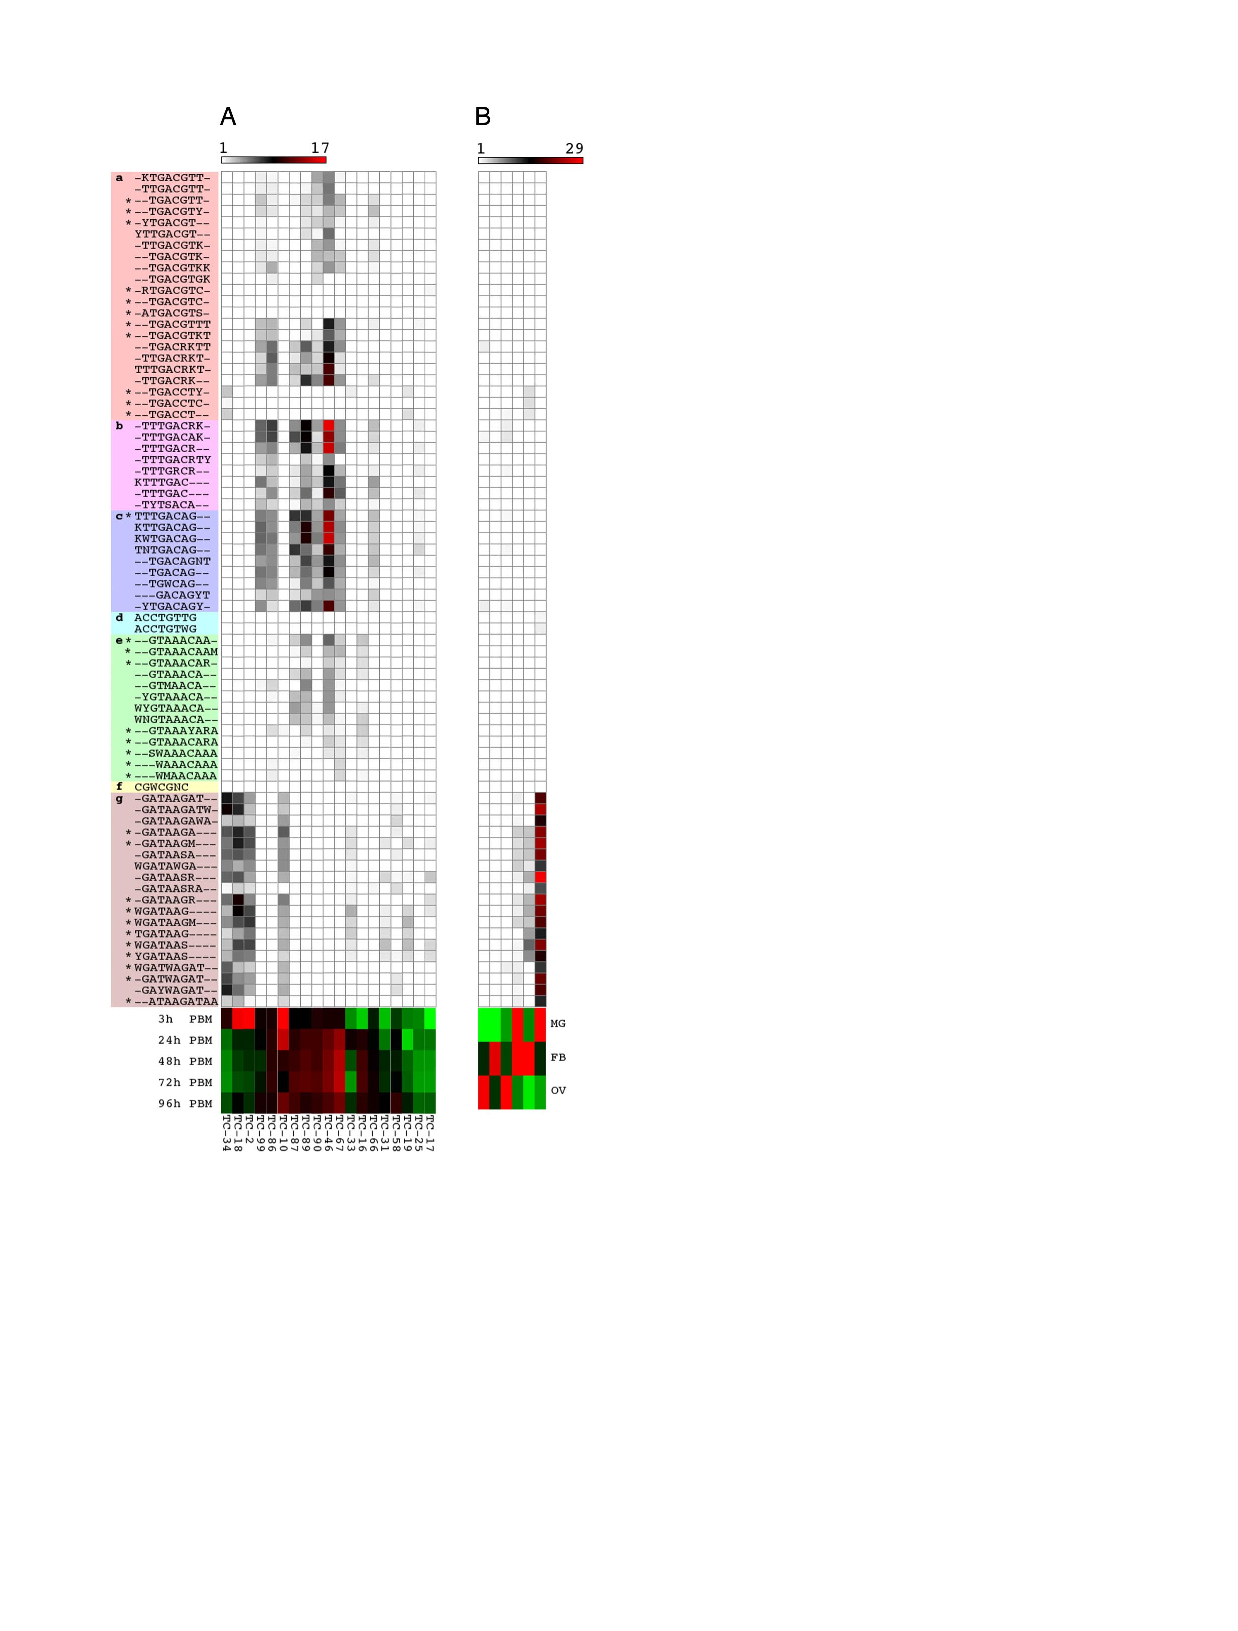
\includegraphics[scale=.95]{figures/figs/sieglaff2009_full.pdf}
\hfil
\caption[Associations of mosquito motifs with gene expression profiles in \Ag]{\bsf{Associations of mosquito motifs with gene expression profiles in \Ag:} \\ \sf
Motif enrichment within (A) 5′-end flanking regions of genes in clusters responsive to blood meal ingestion, and in (B) 5′-end flanking regions of genes in clusters enriched in selected tissues. The significance of motif enrichment is indicated by pseudocolor of -log10 (P-value) determined through hypergeometric statistics, and the median expression profile of each gene cluster is shown below each respective column. Red and green colors represent higher and lower relative mRNA accumulation, respectively. Asterisks (*) indicate a match to a previously described mosquito TFBS. Heatmaps were created with Matrix2png (\CITEME:local-58). FB, fat body; hPBM, hours post blood meal; MG, midgut; OV, ovaries; TC, time course clusters.

Adapted from \cite{Sieglaff2009}}
\label{fig:sieglaff2009_full}
\end{figure}